
Neste capítulo serão desenvolvidos os principais conceitos abordados nos capítulos anteriores. Primeiramente, será feita uma descrição detalhada do problema, incluindo as características das raças Nelore e Caracu, as medidas de interesse (AOL, EGL e EGG), a utilização do TensorFlow/Keras para a implementação do modelo, o processo de aquisição e pré-processamento das imagens de ultrassom e a criação das máscaras de segmentação. Em seguida, serão feitas comparações entre os modelos treinados, utilizando métricas de avaliação adequadas para a tarefa de segmentação de imagens. Duas redes serão implementadas, uma U-Net tradicional e uma U-Net com a integração do sistema de inferência neuro-fuzzy adaptativo (ANFIS), para avaliar o impacto da integração do ANFIS na performance do modelo. 



%O modelo proposto será denominado de \textit{Adaptive Neuro-Fuzzy Inference System for Ultrasound Image Segmentation with U-Net} - ANFIS-UISU (do português, Sistema de Inferência Neuro-Fuzzy Adaptativo para Segmentação de Imagens de Ultrassom com U-Net).
\section{Descrição do Problema}

\subsection{Raças Nelore e Caracu}
A raça Nelore é originária da Índia \cite{hist_nelore}, onde seus ancestrais, os bovinos da raças Ongole, eram criados há milênios por sua rusticidade, resistência a climas tropicais e capacidade de adaptação a ambientes variádos, esses animais foram trazidos ao Brasil no final do século XIX, em um momento de expansão da pecuária nacional. A raça Caracu, por sua vez, tem origem na região da Península Ibérica,chegando no Brasil  logo após o descobrimento, no tempo do Brasil Colônia, os animais da raça Caracu são extremamente funcionais, com alta adaptabilidade e rusticidade, além de serem resistentes a doenças e parasitas \cite{hist_caracu}. O Brasil é um dos maiores criadores mundiais de bovinos da raça Nelore, com uma população estimada em mais de 230 milhões de cabeças \cite{embrapa1}, enquanto a raça Caracu é menos numerosa, mas ainda assim desempenha um papel importante na pecuária brasileira, especialmente em regiões onde a resistência a condições adversas é crucial. \textcolor{red}{parece faltar algo} Uma das principais formas de avaliar o desenvolvimento e a qualidade fenótipa dos animais é por meio da análise de imagens de ultrassom em que, entre outras, é possível obter informações da carcaça do animal. Entre os recursos e metodologias existentes para avaliação de carcaças e de características associadas à qualidade da carne, a ultrassonografia se destaca, especialmente, por possibilitar o exame \textit{in vivo}, uma única vez na vida do animal \cite{cap3:medidaAol}, em tempo relativamente curto, com boa precisão a custos relativamente baixos. O objetivo é conhecer o potencial dos indivíduos e do rebanho como um todo, para musculosidade, precocidade de acabamento e qualidade da carne.

A avaliação é de extrema importância pois existe uma variabilidade nas características que estão relacionadas com a qualidade de desossa, que por sua vez influenciam a comercialização e os resultados econômicos dos produtores \cite{cap3:nelore_caracu}. Dependedo da região do corpo do animal onde a imagem de ultrassom é obtida, é possível extrair diferentes informações, neste trabalho serão utilizadas imagens de ultrassom da região do olho de lombo, que localiza-se entre a 12ª e 13ª costela \cite{cap3:carcaça} e da garupa, como mostra a Figura \ref{fig:regiao_ol}. 
\begin{figure}[H]
    \centering
    \caption{Região do olho de lombo (em amarelo), localizada entre a 12ª e 13ª costela e da garupa (em azul).}
    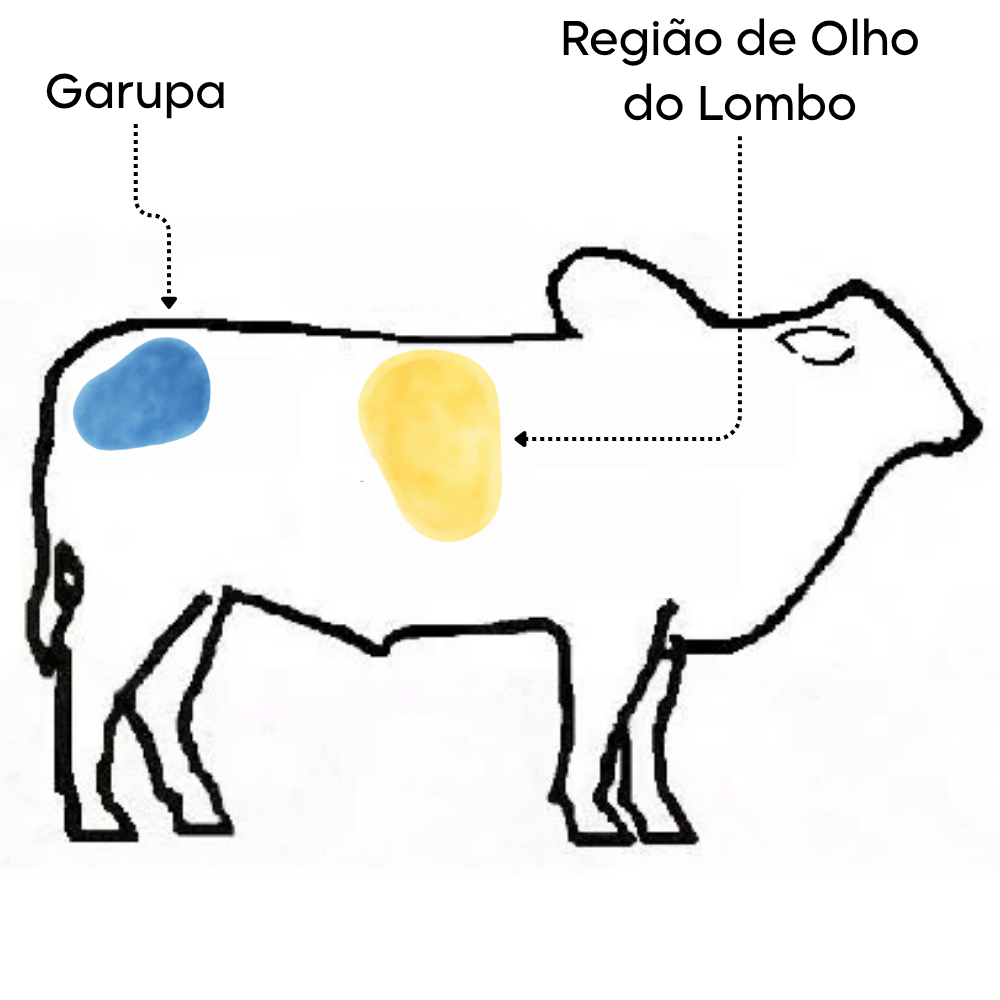
\includegraphics[width=0.5\textwidth]{figures/olho_lombo.png}
    \caption*{Fonte: Adaptado de \cite{cap3:carcaça}.}
    \label{fig:regiao_ol}
\end{figure}
Na região de olho do lombo é possível obter informações de duas medidas importantes para a avaliação da carcaça, a Área de Olho de Lombo (AOL) e a Espessura de Gordura no Lombo (EGL). Na Garupa é possivel obter a Espessura de Gordura na Garupa (EGG). As imagens de ultrassom foram obtidas por meio do aparelho de ultrassom Aloka SSD-500, com todos os animais vivos localizados no Centro Avançado de Pesquisa Tecnológica do Agronegócio em Setãozinho-SP. A Figura \ref{fig1:OL}(a) mostra a imagem do especialista obtendo a imagem de ultrassom da região, já a Figura \ref{fig1:OL}(b) mostra a imagem de ultrassom, a Figura \ref{fig1:OL}(c) mostra a imagem de ultrassom da garupa e a Figura \ref{fig1:OL}(d) mostra o especialista obtendo a imagem de ultrassom da garupa.
\textcolor{red}{esperando elas mandarem as imagens}
\begin{figure}[htpb]
    \centering
    \caption{Aquisição da imagem de ultrassom da região do olho de lombo.}
    \begin{subfigure}{0.45\textwidth}
        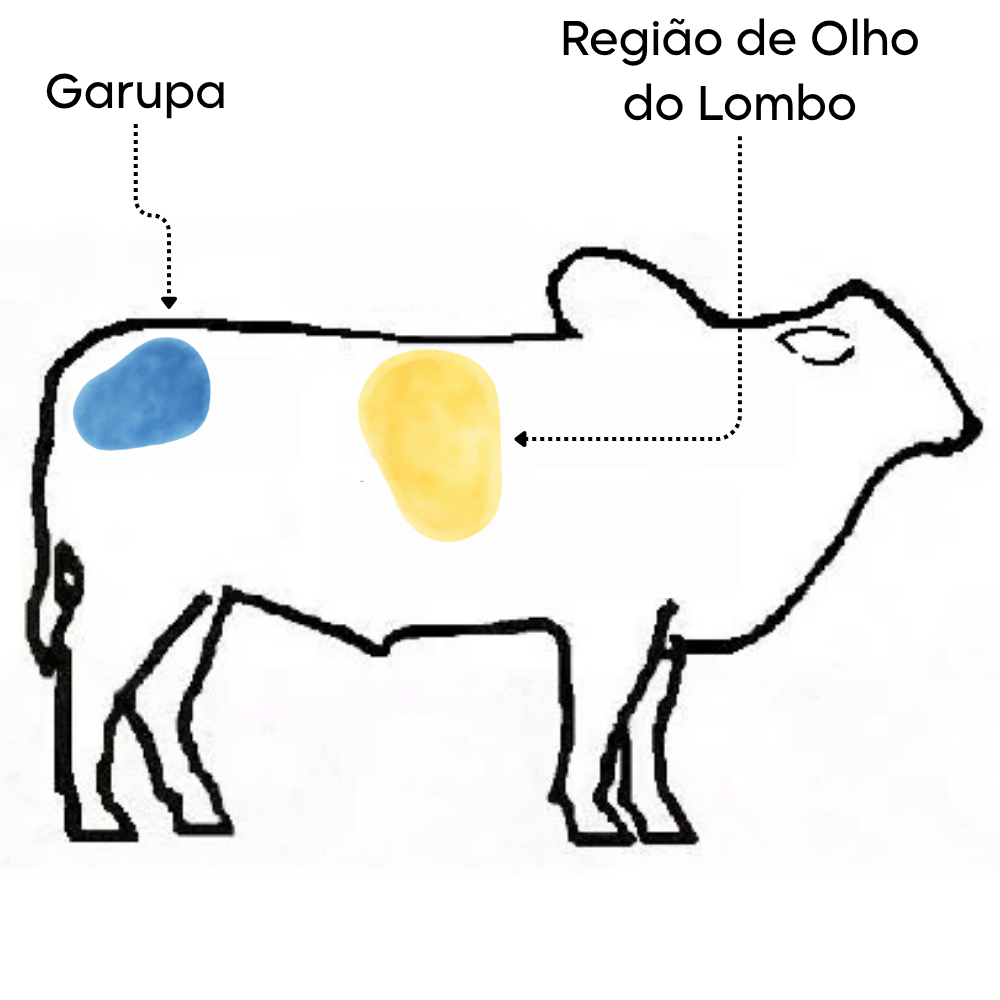
\includegraphics[width=\textwidth]{figures/olho_lombo.png}
        \caption{Especialista obtendo a imagem de ultrassom da região do olho de lombo.}
    \end{subfigure}
    \hfill
    \begin{subfigure}{0.45\textwidth}
        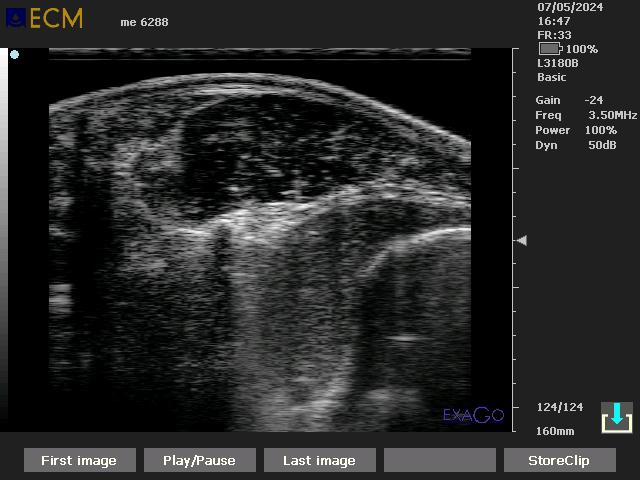
\includegraphics[width=\textwidth]{figures/OL.jpg}
        \caption{Imagem de ultrassom da região do olho de lombo.}
    \end{subfigure}
    \hfill
    \begin{subfigure}{0.45\textwidth}
        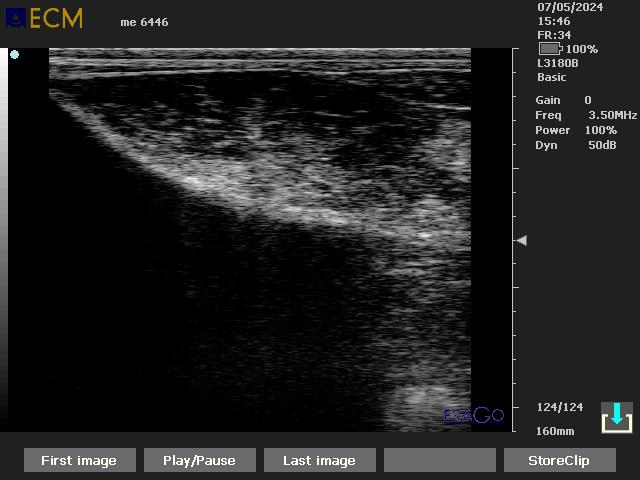
\includegraphics[width=\textwidth]{figures/cap3/EGG.jpg}
        \caption{Imagem de ultrassom da garupa.}
    \end{subfigure}
    \hfill
    \begin{subfigure}{0.45\textwidth}
        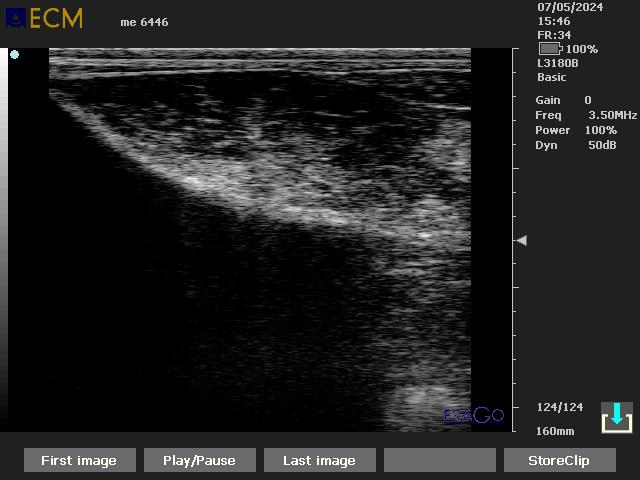
\includegraphics[width=\textwidth]{figures/cap3/EGG.jpg}
        \caption{Especialista obtendo a imagem de ultrassom da garupa.}
    \end{subfigure}
     \caption*{Fonte: Elaboração do Autor.}
     \label{fig1:OL}
\end{figure}



\textcolor{red}{Colocar mais informações}

\subsection{Área de Olho de Lombo (AOL), Espessura de Gordura no Lombo (EGL) e Espessura de Gordura na Garupa (EGG)}
\label{AolEglEgg}
A área de olho de lombo é uma medida que representa a área da seção transversal do músculo  \textit{Longissimus dorsi} (Contrafilé), medida em centímetro quadrados entre a 12ª e 13ª costela. A área está altamente correlacionada com o produto final. Essa característica tem herdabilidade moderada de 35\% e indica musculosidade e rendimento da carcaça \cite{cap3:carcaça}, uma maior área é preferível pelos produtores. Do ponto de vista produtivo, pode-se afirmar que animais com valores de AOL superiores a $75$ cm$^2$, ao abate, apresentam elevados rendimentos de cortes cárneos na indústria figorífica \cite{cap3:medidaAol}. A Figura \ref{cap3:AOL} mostra a demarcação manual da área feita no aplicatvio \textit{ImageJ} \cite{ImageJ} em que a região interna a demarção amarela é a AOL.
\begin{figure}[H]
    \centering
    \caption{Demarcação manual da Área de Olho de Lombo (AOL) utilizando o aplicativo \textit{ImageJ}.}
    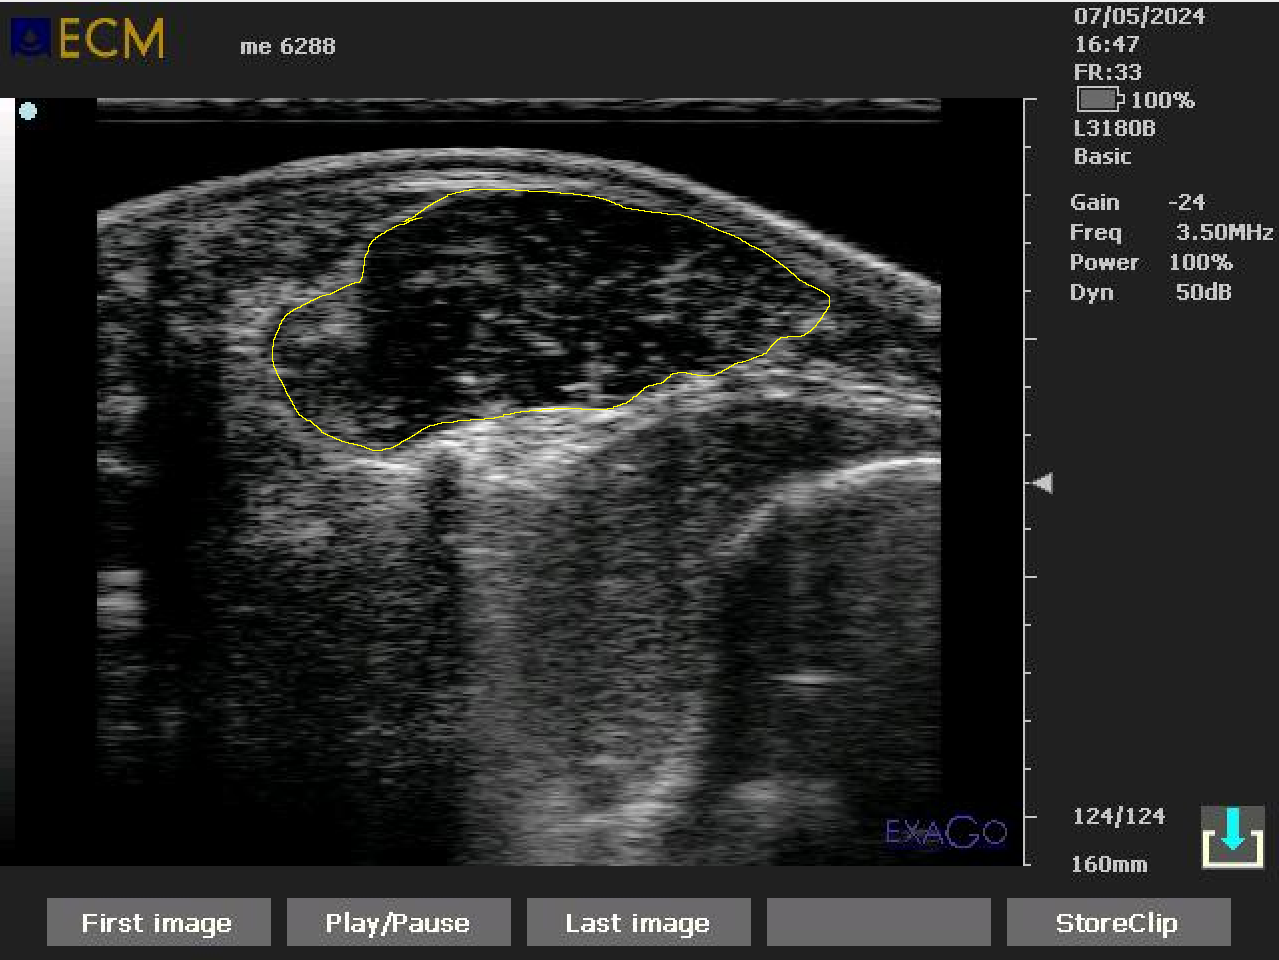
\includegraphics[width=0.7\textwidth]{figures/AOL.png}
    \caption*{Fonte: Elaboração do Autor.}
    \label{cap3:AOL}
\end{figure}

A espessura de gordura no lombo (EGL) é uma medida que representa a espessura da camada de gordura sobre o músculo \textit{Longissimus dorsi} (Contrafilé),  sendo sua espessura (EGL) medida, em milímetros, a $3/4$ da distância medial do músculo, entre a 12ª e 13ª costela. Esta gordura de cobertura é extremamente importante para a proteção da carcaça contra a rápida e intensa queda de temperatura nas câmaras frias, que pode provocar o endurecimento (perda em maciez de até 5 vezes) e o escurecimento da carne em carcaças pobres em acabamento \cite{cap3:medidaAol}. Do ponto de vista de melhoramento genético, a característica da  EGL é um importante indicativo da precocidade sexual e de terminação, ou seja, animais que iniciam a deposição de gordura mais cedo tendem a ser mais precoces, sexualmente, e tendem a apresentar carcaças prontas para o abate em menores idades. Vale ressaltar ainda que EGL apresenta características antagônicas à musculosidade (AOL) e tamanho, ou seja, a seleção exclusiva para precocidade de terminação (EGS) implicará na produção de animais com alta deposição de gordura, mas com menores proporções de cortes cárneos na carcaça e menores pesos ao abate e a idade adulta. A Figura \ref{cap3:EGL} mostra a demarcação manual feita no aplicativo \textit{ImageJ} em que a linha amarela dentro do círculo amarelo representa a demarcação da EGL. 
\begin{figure}[htpb]
    \centering
    \caption{Demarcação manual da Espessura de Gordura no Lombo (EGL) utilizando o aplicativo \textit{ImageJ}.}
    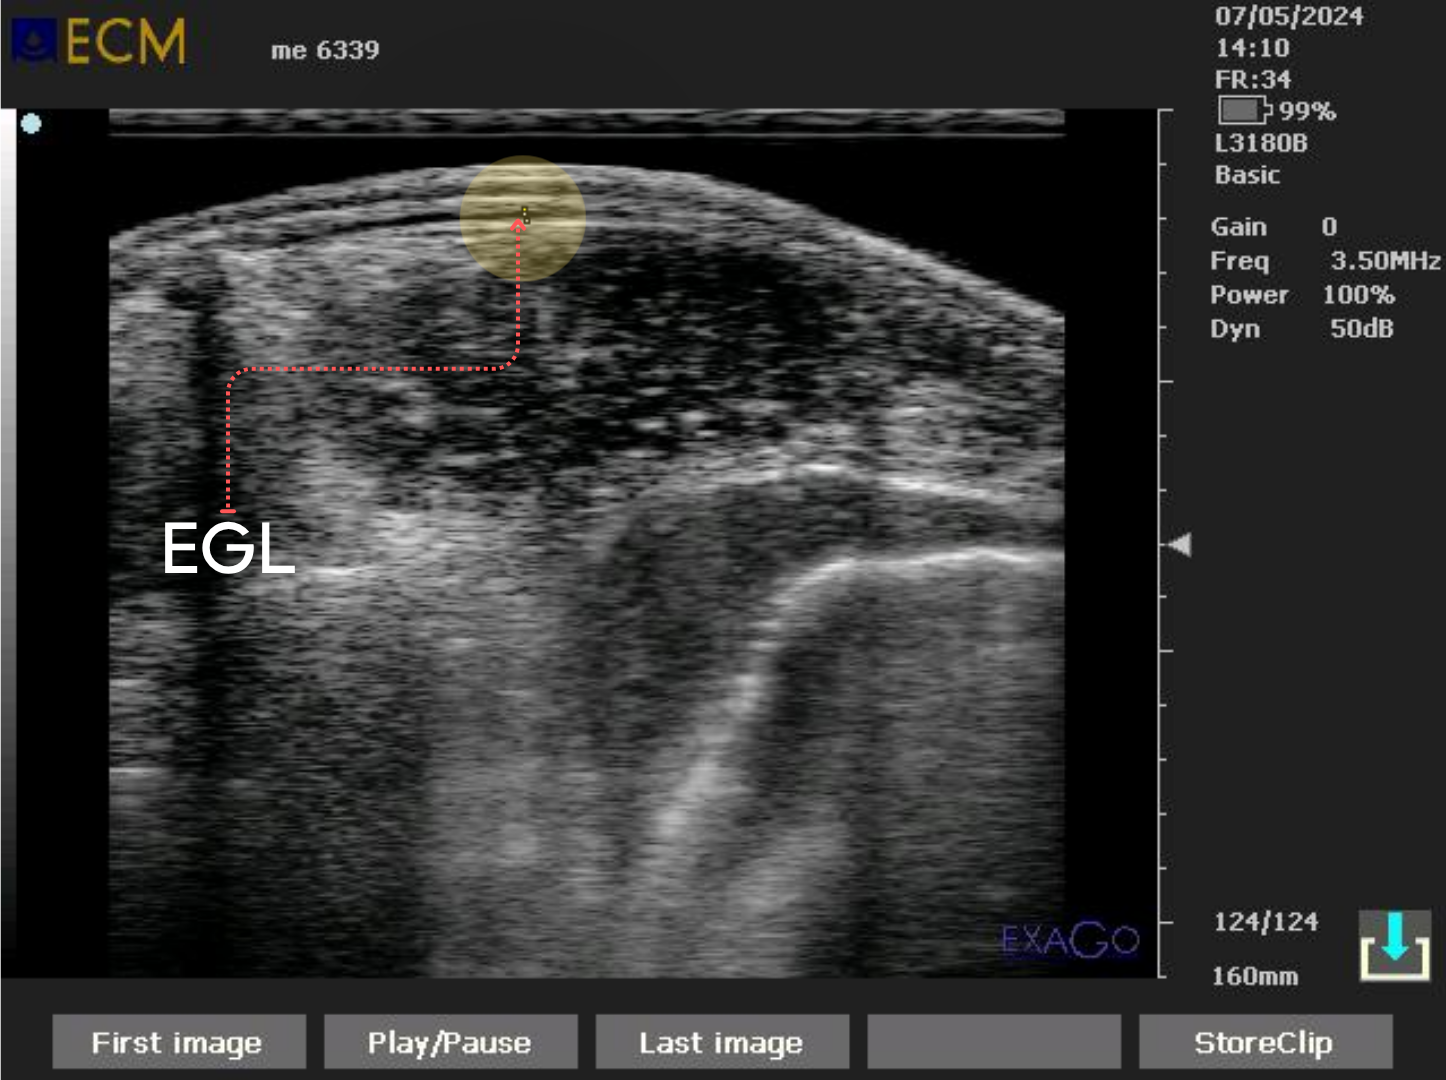
\includegraphics[width=0.8\textwidth]{figures/egl.png}
    \caption*{Fonte: Elaboração do Autor.}
    \label{cap3:EGL}
\end{figure}

A espessura de gordura na garupa (EGG) é uma medida que representa a espessura da camada de gordura sobre a região da garupa, sendo medida em milímetros. A EGG é uma medida complementar à EGL, indicada principalmente para situações em que os animais têm a deposição de gordura subcutânea comprometida, principalmente por nutrição inadequada, como pode ocorrer, por exemplo, com animais em sistemas extensivos de pastejo. Como o processo de deposição de gordura de acabamento inicia-se das extremidades para o centro do corpo, os valores de gordura encontrados na garupa e/ou picanha serão superiores e, consequentemente, minimizam possíveis erros de interpretação dado a baixa variação da medida \cite{cap3:medidaAol}. A medida é obtida observando o músculo \textit{Biceps Femoris}, comumente chamado de ponta da picanha. A Figura \ref{cap3:EGG} mostra a demarcação manual feita no aplicativo \textit{ImageJ} em que a linha amarela dentro do círculo amarelo representa a demarcação da EGG.

\begin{figure}[htpb]
   \centering
   \caption{Demarcação manual da Espessura de Gordura na Garupa (EGG) utilizando o aplicativo \textit{ImageJ}.}
   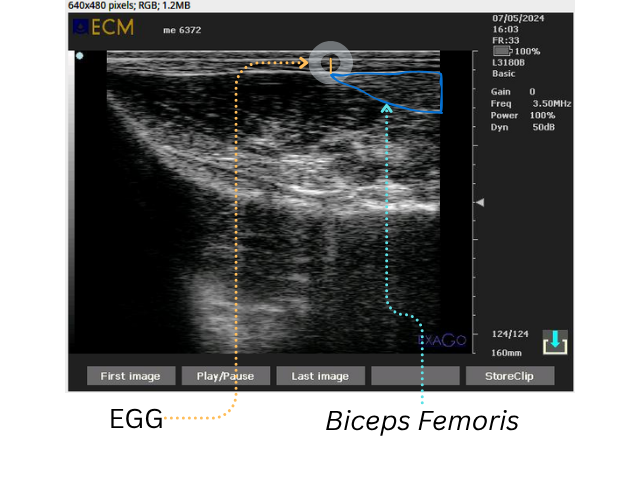
\includegraphics[width=0.8\textwidth]{figures/cap3/medidaEGG.png}
   \caption*{Fonte: Elaboração do Autor.}
   \label{cap3:EGG}
\end{figure}
A espessura é obtida medindo a altura da gordura que encontra-se no começo do \textit{Biceps Femoris} (da esquerda para a direita) \cite{cap3:carcaça}. 
\subsection{Tensorflow/Keras}
O TensorFlow é uma biblioteca de código aberto desenvolvida pelo Google \cite{TensorFlowSite} para computação numérica e aprendizado de máquina. Ele é amplamente utilizado para criar e treinar modelos de aprendizado profundo, incluindo redes neurais convolucionais (CNNs) como a U-Net. O Keras \cite{KerasSite} é uma API de alto nível que roda sobre o TensorFlow, facilitando a construção e o treinamento de modelos de aprendizado profundo. Ele oferece uma interface simples e intuitiva para definir camadas, otimizar modelos e realizar tarefas comuns em aprendizado de máquina. Para este trabalho, utilizaremos o TensorFlow e o Keras para implementar a arquitetura da U-Net e integrar o sistema de inferência neuro-fuzzy adaptativo (ANFIS) para segmentação de imagens de ultrassom. As principais funções e classes do TensorFlow e Keras que serão utilizadas incluem:
\begin{itemize}
    \item \textit{Model}: Classe base para criar modelos personalizados.
    \item \textit{compile}: Função para configurar o modelo para treinamento, especificando o otimizador, a função de perda e as métricas de avaliação.
    \item \textit{fit}: Função para treinar o modelo com os dados de treinamento.
    \item \textit{evaluate}: Função para avaliar o desempenho do modelo com os dados de teste.
    \item \textit{predict}: Função para fazer previsões com o modelo treinado.
    \item \textit{Input}: Função para definir a entrada do modelo.
    \item \textit{Conv2D}: Camada de convolução bidimensional para extrair características das imagens.
    \item \textit{MaxPooling2D}: Camada de \textit{pooling} para reduzir a dimensionalidade das características extraídas.
    \item \textit{Conv2DTranspose}: Camada de convolução transposta para realizar a operação de espansão da imagem na arquitetura da U-Net.
    \item \textit{Concatenate}: Função para concatenar as camadas de características durante a fase de expansão da U-Net.
    \item \textit{Dense}: Camadas com unidades totalmente conectadas, especialmente útil para a parte de \textit{Multitask} da U-Net.
    \item \textit{Reshape}: Função para transformar a dimensão dos dados.
    \item \textit{Dropout}: Camada para regularização do modelo, ajudando a prevenir o \textit{overfitting}.
\end{itemize}
\subsection{Aquisição e Pré-processamento das Imagens}
As imagens de ultrassom foram adquiridas utilizando o aparelho Aloka SSD-500, com os animais vivos localizados no Centro Avançado de Pesquisa Tecnológica do Agronegócio em Setãozinho-SP. No total foram enviadas $135$ imagens de ultrassom, sendo $108$ imagens da raça Nelore e $27$ imagens da raça Caracu. As imagens foram divididas em conjuntos de treinamento ($70\%$), validação ($20\%$) e teste ($10\%$). Por conta da quantidade de imagens ser extremamente baixa para o treinamento de um modelo de aprendizado profundo, foi necessário realizar um processo de aumento de dados (\textit{data augmentation}) para aumentar a quantidade de imagens disponíveis para o treinamento além de um corte nas imagens para a remoção de informações irrelevantes durante o treinamento e que poderiam enviesar o modelo, prejudicando seu desempenho. O processo de aumento de dados incluiu as seguintes transformações:
\begin{itemize}
    \item Rotação: As imagens foram rotacionadas em ângulos dentro do intervalo de $[-15^\circ, 15^\circ]$ para criar variações na orientação das imagens.
    \item Aumento e redução de brilho: As imagens foram aumentadas e reduzidas em brilho para simular diferentes condições de iluminação.
\end{itemize}
Todas as modificações feitas foram realizadas observando as características das imagens de ultrassom presentes no banco de dados. Como cada imagem foi modificada três vezes, o processo de aumento de dados resultou em um total de $376$ imagens para o treinamento do modelo, pois $70\% \times 134 = 94$ e $94 \times 3 = 282  + 94 = 376$. O pré-processamento das imagens incluiu a normalização dos valores dos pixels para o intervalo $[0, 1]$ e o redimensionamento das imagens para um tamanho fixo de $256 \times 256$ pixels, garantindo que todas as imagens tivessem a mesma dimensão para o treinamento do modelo. Além disso, as máscaras de segmentação foram criadas manualmente, com a ajuda de uma especialista, utilizando a biblioteca do Python, \textit{label studio} \cite{LabelStudioSite} \textcolor{red}{precisa da data já que é site?}, em que as regiões correspondentes à AOL, EGL e EGG foram demarcadas para serem utilizadas como ``rótulos" durante o treinamento do modelo. A Figura \ref{cap3:preprocessamento} mostra um exemplo do processo de pré-processamento.
\begin{figure}[H]
    \centering
    \caption{Exemplo do processo de pré-processamento das imagens de ultrassom.}
    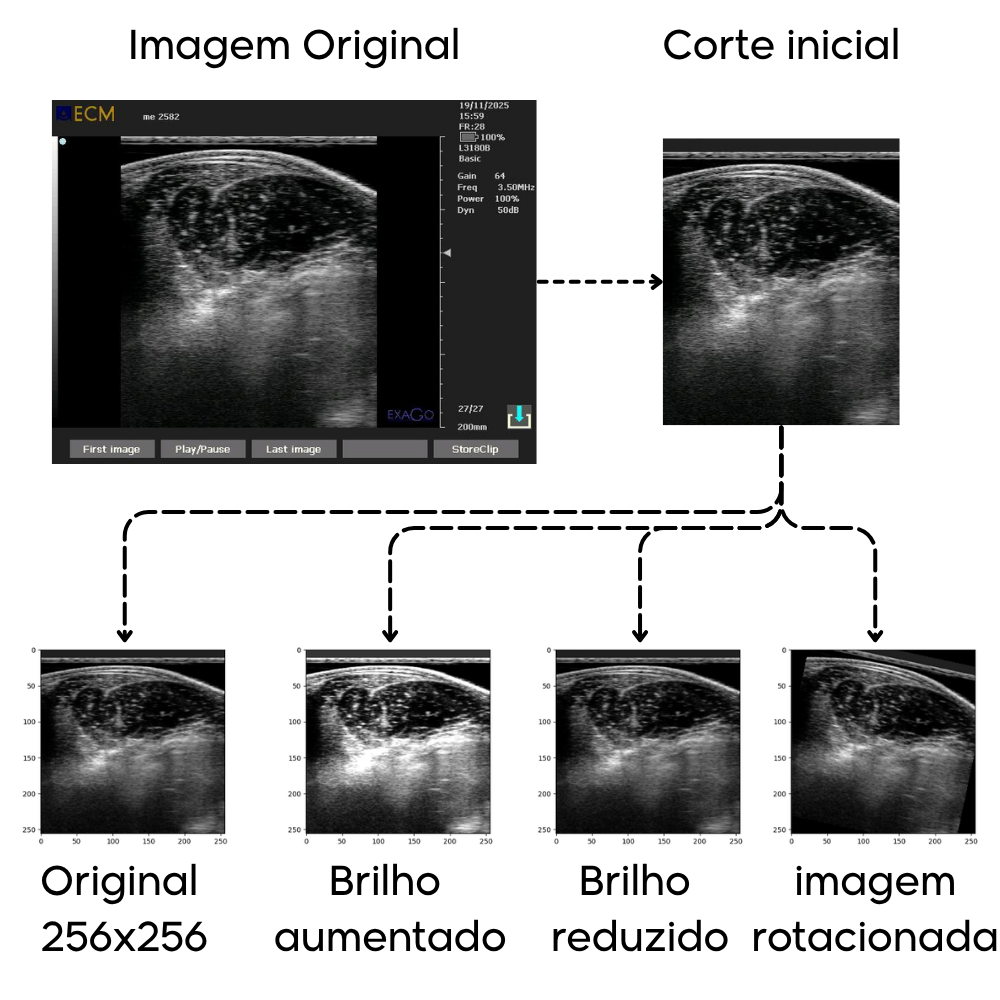
\includegraphics[width=0.7\linewidth]{figures/cap3/augmentation.png}  
    \caption*{Fonte: Elaboração do Autor.}
    \label{cap3:preprocessamento}  
\end{figure}

\subsection{Máscaras}
Cada medida presente nas imagens de ultrassom são números reais, por exemplo, a AOL é medida em centímetros quadrados, a EGL e a EGG são medidas em milímetros. Uma ideia inicial foi desenvolver uma rede que recebia as imagens de ultrassom e retornava como saída os valores numéricos correspondentes à AOL, EGL e EGG, ou seja, uma rede de regressão. No entanto, devido à quantidade extremamente baixa de imagens disponíveis para o treinamento do modelo, foi necessário realizar uma adaptação na abordagem inicial. Em vez de treinar um modelo de regressão para prever os valores numéricos das medidas, optou-se por criar máscaras de segmentação para cada medida (AOL, EGL e EGG) a partir das imagens de ultrassom. As máscaras de segmentação da AOL foram criadas demarcando a região correspondente à área do músculo, as máscaras de segmentação da EGL foram criadas demarcando a região correspondente à camada de gordura sobre o músculo \textit{Longissimus dorsi} e as máscaras de segmentação da EGG foram criadas demarcando a região correspondente à camada de gordura sobre a região da garupa e demarcadando o músculo \textit{Biceps Femoris} pois, a medida da EGG acontece em um local específico da imagem.

Foram treinados quatro modelos, um para cada medida, dois modelos para as máscaras da EGG. Após o treinamento, a saída do modelo é processada para extrair as medidas numéricas correspondentes. Para a AOL, a área da região segmentada é calculada e convertida para centímetros quadrados. Para a EGL, a espessura da camada de gordura é medida a partir de $3/4$ da região segmentada e convertida para milímetros. Para o EGG, a espessura da camada de gordura é medida como mostra a subseção \ref{AolEglEgg}. Essa abordagem permitiu contornar a limitação de dados e ainda assim obter as medidas numéricas desejadas a partir das imagens de ultrassom. 
As máscaras de segmentação estão em preto e branco, onde as regiões em branco representam as áreas de interesse (AOL, EGL e EGG) e as regiões em preto representam o fundo da imagem. A Figura \ref{cap3:mascaras} mostra um exemplo das máscaras de segmentação criadas para as imagens de ultrassom.
\begin{figure}[H]
    \centering
    \caption{Exemplo das máscaras de segmentação criadas para as imagens de ultrassom.}
    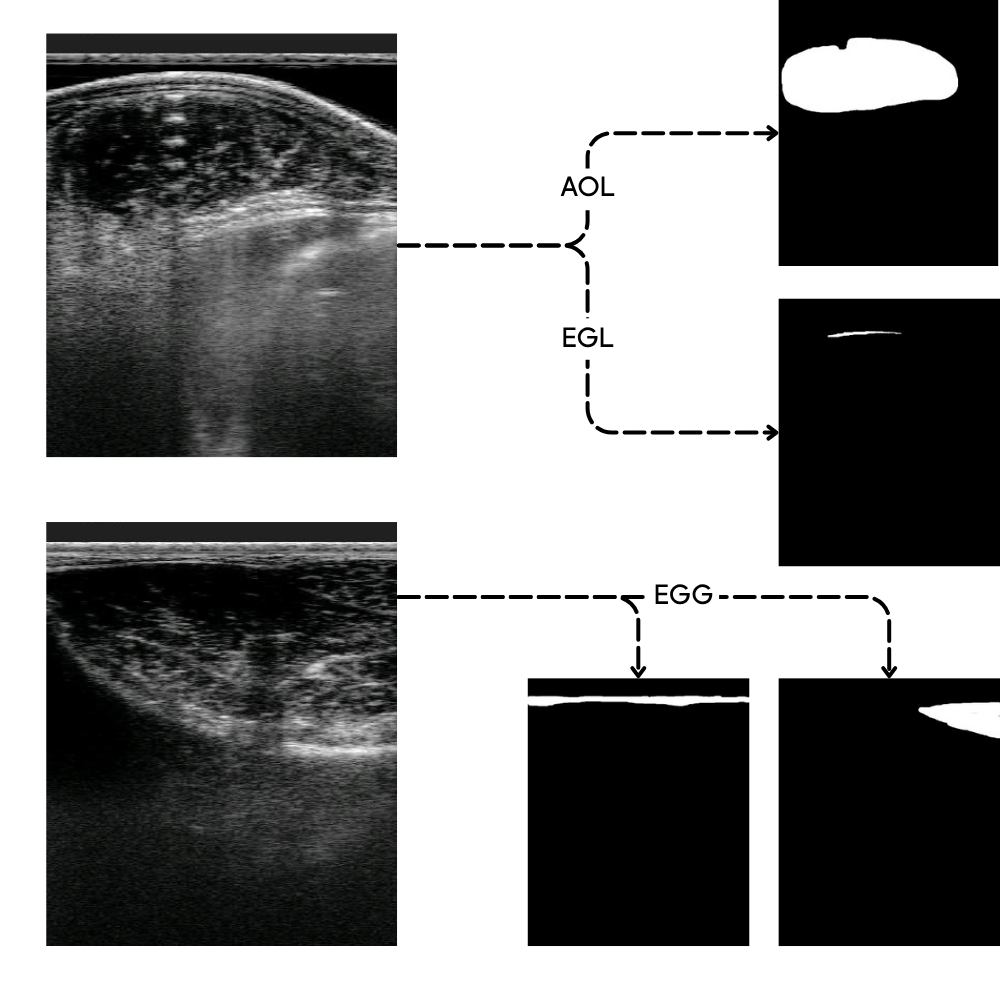
\includegraphics[width=0.7\linewidth]{figures/cap3/mascaras.png}  
    \caption*{Fonte: Elaboração do Autor.}
    \label{cap3:mascaras}
\end{figure}

Cada imagem de animal vinha com um número de indentificação, como pode ser visto em cada uma das Figuras \ref{fig1:OL}, \ref{cap3:AOL}, \ref{cap3:EGL} e \ref{cap3:EGG}, no canto superior esquerdo (começando com ``me"). Animais com o primeiro dígito começando em $6$, são animais da raça Nelore, enquanto animais com o primeiro dígito começando em $2$, são animais da raça Caracu. Essa indentificação serviu para terminar o desenvolvimento dos dados e criar as variáveis de entrada da rede no pardrão visto na seção \ref{multitask}, ou seja, cada variável de entrada da rede será composta por uma imagem de ultrassom e a raça do animal correspondente à imagem, sendo codificada no formato \textit{One-Hot Encoding}, em que a raça Nelore é representada por $[1, 0]$ e a raça Caracu é representada por $[0, 1]$.

\section{U-Net e U-Net \textit{Multitask} com inferência Fuzzy}

\subsection{Treinamento e Métricas de Avaliação}
Como foram desenvolvidos quatro modelos, o processo de treinamento foi realizado separadamente para cada modelo. O treinamento incluiu a definição da arquitetura da U-Net, a configuração dos hiperparâmetros do modelo, a escolha da função de perda e do otimizador, e a execução do processo de treinamento utilizando os dados de treinamento e validação. Cada medida (AOL, EGL e EGG) teve dois modelos, um modelo U-Net com modificações e um modelo de U-Net com a integração do sistema de inferência neuro-fuzzy adaptativo (ANFIS). 
\begin{itemize}
    \item U-Net: Algumas modificações foram feitas no modelo original proposto por \cite{Ronneberger2015UNet}, sendo elas:
    \begin{itemize}
        \item  No \textit{encoder} a rede é divida em blocos, cada bloco é composto por duas camadas de convolução (\textit{Conv2D}) com \textit{kernels} de tamanho $3\times 3$, \textit{stride} de tamanho $1$, \textit{padding} ``\textit{same}" e função de ativação ReLU, seguidas por uma camada de \textit{MaxPooling} para reduzir a dimensionalidade da imagem com \textit{kernel} de tamanho $2\times 2$, \textit{stride} de tamanho $2$ e \textit{padding} ``\textit{same}". No total foram 4 blocos no \textit{encoder}, com o número de filtros dobrando a cada bloco, começando com $64$ filtros no primeiro bloco e chegando a $512$ filtros no quarto bloco.
        
        \item  No \textit{baseline} tem-se duas camadas de convolução (\textit{Conv2D}) com \textit{kernel} de tamanho $3\times 3$, \textit{stride} de tamanho $1$, \textit{padding} ``\textit{same}" e função de ativação ReLU.
        
        \item Para levar em consideração a raça do animal é adicionada uma camada \textit{Multitask} na parte de \textit{baseline} da U-Net, de forma silimar a vista na subseção \ref{multitask}.
        
        \item  No \textit{decoder} a rede também é divida em blocos, cada bloco é composto por uma camada de convolução transposta (\textit{Conv2DTranspose}) com \textit{kernel} de tamanho $2\times 2$, \textit{stride} de tamanho $2$ e \textit{padding} ``\textit{same}", seguida por uma camada de concatenação para concatenar as características extraídas pelo \textit{encoder} com as características extraídas pelo \textit{decoder}, seguida por uma camada de convolução (\textit{Conv2D}) com \textit{kernel} de tamanho $3\times 3$, \textit{stride} de tamanho $1$, \textit{padding} ``\textit{same}" e função de ativação ReLU. No total foram 4 blocos no \textit{decoder}, com o número de filtros reduzindo pela metade a cada bloco, começando com $512$ filtros no primeiro bloco e chegando a $64$ filtros no quarto bloco. A camada de saída é composta por uma camada de convolução (\textit{Conv2D}) com um único filtro, \textit{kernel} de tamanho $1\times 1$, \textit{stride} de tamanho $1$, \textit{padding} ``\textit{same}" e função de ativação \textit{Sigmoid} para produzir a máscara de segmentação.
    \end{itemize}
    A Figura \ref{dimensoesIMG} mostra a arquitetura da U-Net utilizada e como as dimensões das imagens vão se modificando ao longo da rede.
    \begin{figure}[H]
        \centering
        \caption{Arquitetura da U-Net utilizada e as dimensões das imagens ao longo da rede.}
        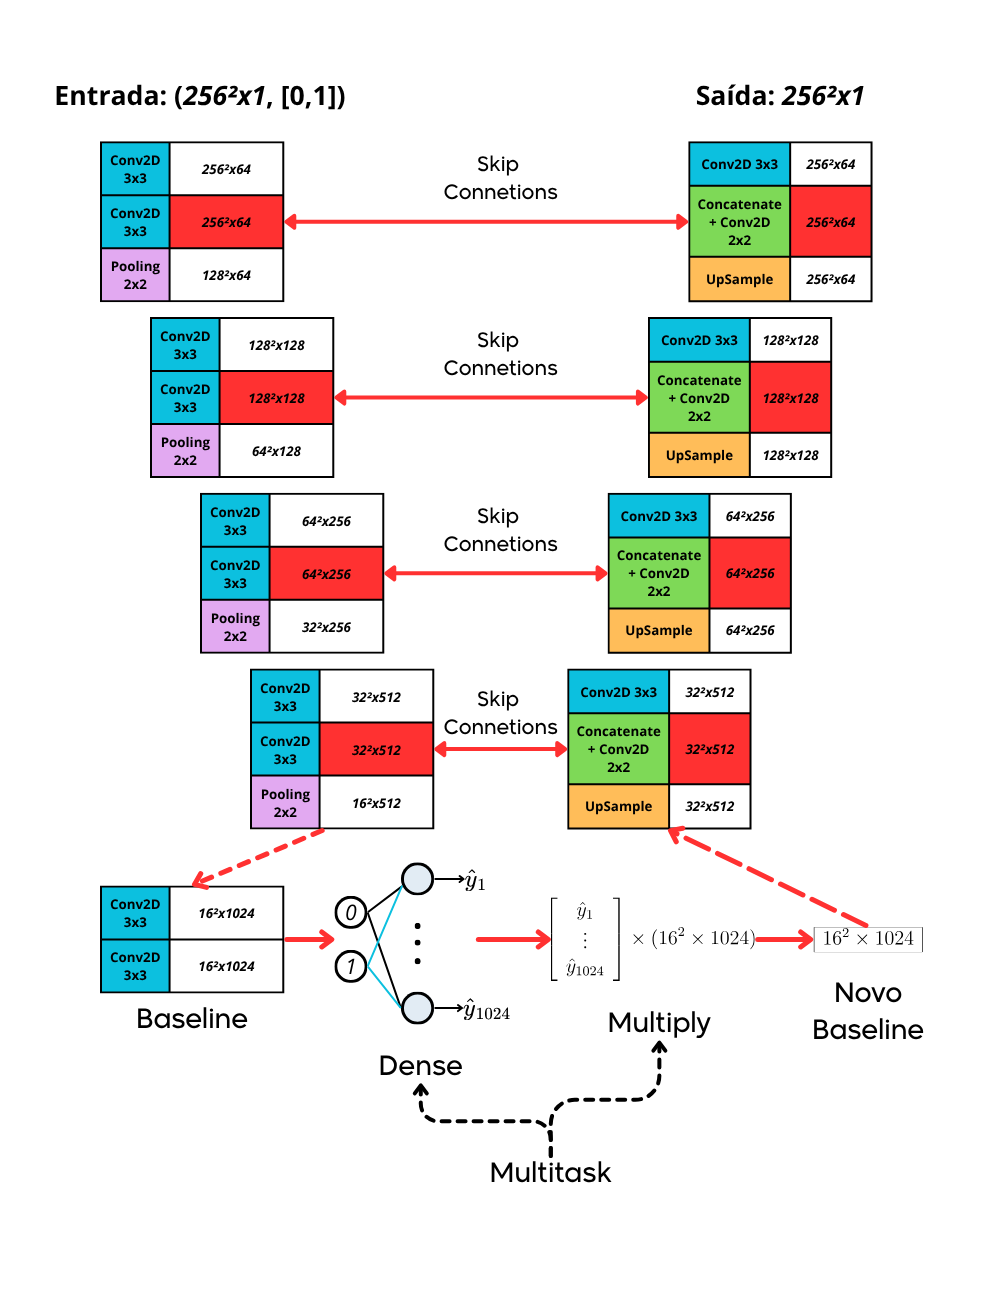
\includegraphics[width=0.8\textwidth]{figures/cap3/imgdimensoes.png}  
        \caption*{Fonte: Elaboração do Autor.}
        \label{dimensoesIMG}
    \end{figure}
    A cor azul representa as camadas de convolução com filtros de tamanho $3\times 3$,a cor roxa representa as camadas de \textit{MaxPooling}, a cor laranja representa as camadas de convolução transposta (\textit{UpSample}) com filtros de tamanho $2\times 2$ e a cor verde representa as camadas de concatenação e convoluções com filtros de tamanho $2\times 2$. As setas indicam o caminho dos dados ao longo da rede, mostrando como as características extraídas pelo \textit{encoder} são concatenadas com as características extraídas pelo \textit{decoder} (\textit{Skip Connection}) para produzir a máscara de segmentação final. O \textit{Multitask} após o \textit{baseline} e a representação visual das equações vistas na subseção (\ref{multitask}), com \textit{Dense} e \textit{Multiply} sendo as funções do \textit{Tensorflow} utilizadas para criar a camada.

    Em todos os blocos foram adicionadas camadas de \textit{Dropout} com uma taxa de $0.1$ para regularização do modelo e prevenir o \textit{overfitting}. O modelo foi treinado utilizando o otimizador Adam, com uma taxa de aprendizado inicial de $0.001$, um número máximo de épocas definido em $100$ e função de custo sendo a \textit{Binary Cross-Entropy} (BCE). O processo de treinamento foi monitorado utilizando os dados de validação com o \textit{EarlyStopping} para evitar também o \textit{overfitting} e garantir a generalização do modelo. 

    \item U-Net \textit{Multitask} com inferência Fuzzy: Como comentado na subseção (\ref{multitask}) a U-Net \textit{Multitask} com inferência Fuzzy compartilha quase todos as definições da U-Net tradicional (\textit{encoder} e \textit{decoder} iguais), entretanto, o \textit{baseline} é alterado para incluir mais uma modificação importante, a integração do sistema de inferência neuro-fuzzy adaptativo (ANFIS). Com isso, algumas variáveis extras precisam ser definidas:
    \begin{itemize}
        \item Número de Conjuntos Fuzzy: O número de conjuntos fuzzy para cada variável de entrada do ANFIS foi definido como $3$, ou seja, ``Baixo", ``Médio" e ``Alto". 
        \item Número de Regras Fuzzy: O número de regras fuzzy foi definido como $9$, considerando todas as combinações possíveis dos conjuntos fuzzy para a variável de entrada (características extraídas pelo \textit{baseline} da U-Net \textit{Multitask}).
    \end{itemize}
\end{itemize}